\section{Models}
In this work we take in consideration some SOTA models for camera pose estimation, also adding small modifications to make them fit better to our use case scenario.
In particular, we present:
\begin{itemize}
    \item MeNet (add citation) for RPE;
    \item PoseNet~\cite{9348762} and MapNet~\cite{DBLP:journals/corr/abs-1712-03342} for APE.
\end{itemize}

\subsection{MeNet}
The first model we would like to analyze is the MeNet model (\cref{fig:menet-structure}), which is specifically targeted for RPE.
The input of the network consists in a stack of two images: the goal is to estimate the relative pose of the second image with respect to the first one.
As presented in \cref{fig:menet-structure}, the MeNet is composed by nine deep convolutional layers followed by a pair of linear layers. While the first part of the network works as a feature extraction mechanism, the last layers are used to combine the extracted features.
\begin{figure}
    \begin{center}
        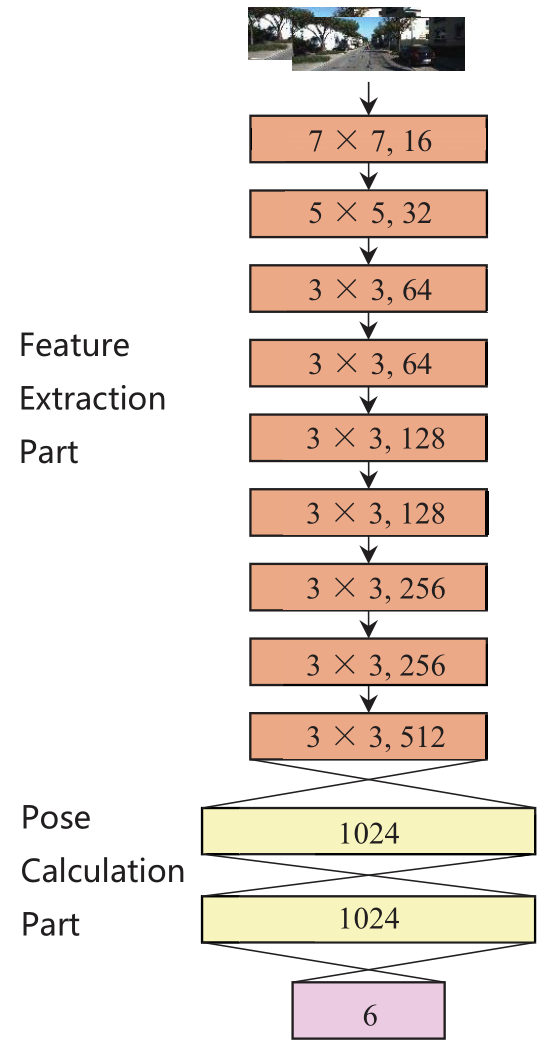
\includegraphics[width=0.32\textwidth]{./imgs/menet_structure.png}
    \end{center}
    \caption{The architecture of the MeNet model.}
    \label{fig:menet-structure}
\end{figure}

In order to train the model, we use a loss function that consists in the weighted composition of two Mean Square Errors (MSE) computed separately on positions and quaternions:
\begin{equation}
    Loss(w) = \frac{1}{N} \sum\limits_{i=1}^N \norm{P^i - \hat{P}^i}^2_2 + \alpha\norm{Q^i - \hat{Q}^i}^2_2
    \label{eq:menet-loss}
\end{equation}
where $P$, $\hat{P}$, $Q$, $\hat{Q}$, and $\alpha$ are the ground truth position vector, the estimated position vector, the ground truth quaternions, the estimated quaternions, and the weight for balancing the displacement error and the rotation angle error.

\subsection{PoseNet}
Since the results given by RPE deep learning solutions are not very promising, from now on we are going to consider models strictly developed for APE.
In this sense, the first model we present is the PoseNet model~\cite{9348762}.
Just like the MeNet model, the PoseNet is made up by two components:
\begin{itemize}
    \item feature extraction through a sequence of convolutional layers. This component has been named internally also as \emph{backend};
    \item pose regression on the extracted features using linear layers.
\end{itemize}
This model architecture is actually pretty convenient, since it can use pre-trained deep convolutional models, through the transfer learning approach. In most of the cases, this kind of models are trained on the ImageNet dataset \cite{imagenet}, which counts almost 3.2 million real-world images. Some examples of SOTA backend models that have been considered are: GoogLeNet~\cite{googlenet}, ResNet~\cite{resnet}, and EfficientNet-B7~\cite{efficientnet}. \Cref{tab:backend-performance-imagenet} shows the accuracy over the k=(1, 5) top predictions for the used backends on the ImageNet dataset.

\begin{table}[htbp]
    \caption{Backends performance in ImageNet}
    \begin{center}
        \begin{tabular}{lrr}
            \toprule
            Model           & Acc@1           & Acc@5           \\
            \midrule
            GoogLeNet       & 69.778          & 89.530          \\
            ResNet-18       & 69.758          & 89.078          \\
            ResNet-34       & 73.314          & 91.420          \\
            ResNet-50       & 76.130          & 92.862          \\
            ResNet-152      & 78.312          & 94.046          \\
            EfficientNet-B7 & \textbf{84.122} & \textbf{96.908} \\
            \bottomrule
        \end{tabular}
        \label{tab:backend-performance-imagenet}
    \end{center}
\end{table}

Since ImageNet pre-trained models are used for classification purposes, we can just remove the last layers, and use only the feature extraction-related ones. In this way we are introducing in the PoseNet a feature extraction mechanism on real-world images with minimum effort: training by scratch these models would require a huge amount of computational power.

Also in this model we adopt the weighted loss described in \cref{eq:menet-loss}, also used in the MeNet model.

\subsection{MapNet}
The MapNet model for APE represents an evolution of the PoseNet model: in fact, the model architecture remains actually the same. On the contrary, the main difference between the PoseNet is the loss function used to train the model. In this case, the errors in the prediction of absolute poses are not the only ones which are penalized: also errors in the relative poses are taken in consideration.

The size of the last linear block depends on the dimension of the map that we would like to introduce.
